% !TEX program = xelatex
\documentclass[11pt]{article}
\usepackage[a4paper,top=0.8in,bottom=0.8in]{geometry}
\usepackage[labelfont=bf,labelsep=quad]{caption}
\usepackage[UTF8]{ctex}
\usepackage{multirow,booktabs}
\usepackage{relsize,bm,amsmath,amsfonts,amssymb}
\usepackage{subfigure,graphicx}
\usepackage{enumitem}
\usepackage{listings,color}
\usepackage{hyperref}
\hypersetup{
    colorlinks,
    linkcolor=black,
    filecolor=black,      
    urlcolor=blue,
    citecolor=black,
}
\definecolor{dkgreen}{rgb}{0,0.6,0}
\setCJKmainfont{FangSong}[AutoFakeBold = {3}]
\renewcommand\thesection{\Roman{section}}
\renewcommand\thesubsection{\arabic{section}.\arabic{subsection}}

\begin{document}
\begin{center}
    \bf{\zihao{3}实验报告 \quad {金融新实体发现}}
\end{center}

\vspace{-5mm}
\section{问题定义}\label{Theory}
\vspace{-2mm}
随着互联网技术的不断发展,如何对飞速增长的互联网文本中包含的知识进行高效可靠的挖掘并进行组织,已成为自然语言处理(NLP)和信息抽取研究中的重要目标。%
互联网中各种命名实体及之间的关系纷繁复杂,单纯地以人工和经验的方式进行相关知识的获取及组织已经远远不能满足人们的使用要求。为此,知识的自动%
获取逐渐地成为文本处理的重要课题。针对这一问题,金融实体识别方案的建立将极大提高金融信息获取效率,从而更好的为金融领域相关机构和个人提供信息支撑。\par

命名实体识别(Named Entity Recognition,简称NER),是指识别文本中具有特定意义的实体,主要包括人名、地名、机构名、专有名词等。%
图\ref{illustration_ner} 展示了从英文文本中进行实体识别的一个例子。

\begin{figure}[!ht]
    \centering
    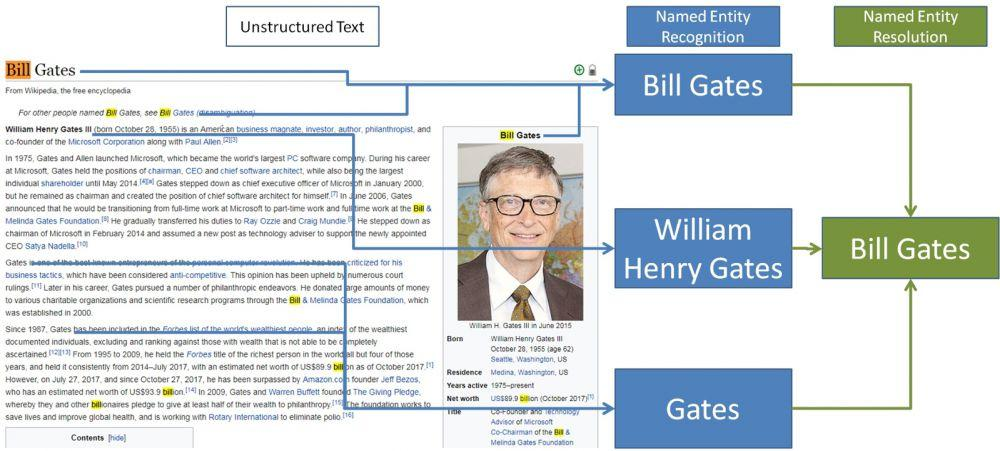
\includegraphics[height=2in]{pic/NER.jpg}
    \caption{命名实体识别实例}
    \label{illustration_ner}
\end{figure}

NER通常包括两部分:(1)实体边界识别;(2) 确定实体类别(人名、地名、机构名或其他)。实体边界识别指从一个句子中分辨出一个个的词,%
确定实体类别则是指将分辨出来的词归类到不同的类别中。中文命名实体识别主要有如下几种方法,适用于不同的场景:

\begin{enumerate}
    \item 基于规则和词典的方法。基于规则的方法多采用构造规则模板,以模式和字符串相匹配为主要手段。显而易见,对于新出现的实体,想要设计通用的字典进行匹配几乎是不可能的。
    \item 基于统计的方法。传统统计机器学习的方法有很多,常见的包括HMM, SVM, CRF等。这些方法比较依赖于语料库。
    \item 基于深度学习的方法。深度学习已经在NLP的很多领域取得了巨大的成功。尽管算法面临着诸多挑战,如计算资源开销大、依赖数据量及其标注,但模型的性能较之过去有了很大的提升。
\end{enumerate}


本次实验基于BDCI 2019的相关赛题,借鉴了Google Bert模型。实验报告将围绕数据集分析、算法实现以及实验结果等这几部分展开。

\section{数据集分析与处理}
\subsection{数据集简介}
实验处理的是互联网金融新实体数据来自BDCI官方提供的赛题数据,数据类型是中文自然语言处理文本,主要是自动爬取的金融网络文本,包括标题和内容,并进行了简单的标注和转换。数据规模上,训练集数据量和测试集数据量都是一万条文本数据。%
训练数据全部以csv格式给出。其文件是一个字符序列。每条数据包括标识号(id)、文本标题(title)、文本内容(text)、未知实体列表(unknownEntities)。每条数据的内容如表\ref{data_description} 所示。
%
\tabcolsep=12pt
\begin{table}[!ht]
    \centering
    \begin{tabular}{llll}
        \toprule
        字段类型 & 类型 & 描述 & 数据集实例\\ \midrule
        id & String & 数据ID & 2e6a5020 \\
        title & String & 文本标题 & 人人都在用手机赚钱\\
        text & String & 文本内容 & 比如做微商,做代理……\\
        UnknownEntities & String & 未知实体列表 & 趣投美元 \\ 
        \bottomrule
    \end{tabular}
    \caption{数据格式说明}
    \label{data_description}
\end{table}

\subsection{数据集缺陷}
由于数据是直接从网络文段中自动爬取的,只是经过了简单的标注和处理,所以会存在一些问题。与所有传统的数据挖掘(Data Mining)任务相似,该数据集也并非尽善美。经过初步的预分析,结果表明数据在如下方面有进一步完善的可能性:
\begin{enumerate}[label=(\roman*)]
    \item 存在html标记语言、IMG转换标记、非文字字符与混乱字符以及大量重复的字符。如图\ref{p1} 所示。
    \item 部分数据内容相似性度高,甚至完全重复。很多数据标题和内容也是高度一致的。如图\ref{p2} 所示。
    \item 标签混淆文本,缺乏实质性意义。如图\ref{p3} 所示。
    \item 人工标注存在问题。如一些知名企业仍标注为未知实体。如图\ref{p4} 所示。
\end{enumerate}


\vspace{-4mm}
\begin{figure}[!ht]
    \centering
    \subfigure[符号问题]{
        \begin{minipage}[t]{\linewidth}
            \centering
            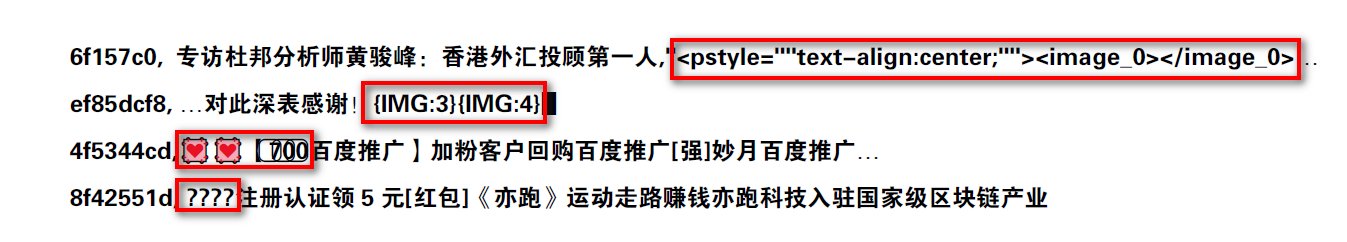
\includegraphics[width=\linewidth]{pic/prob1.png}
            \label{p1}
        \end{minipage}
    }

    \subfigure[重复文本数据]{
        \begin{minipage}[t]{\linewidth}
            \centering
            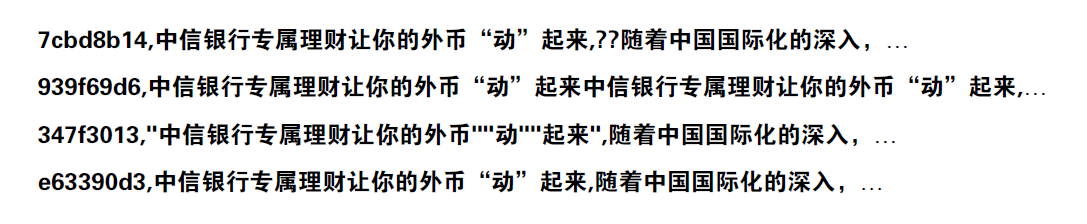
\includegraphics[width=\linewidth]{pic/prob2.png}
            \label{p2}
        \end{minipage}
    }

    \subfigure[标签混入文本]{
        \begin{minipage}[t]{\linewidth}
            \centering
            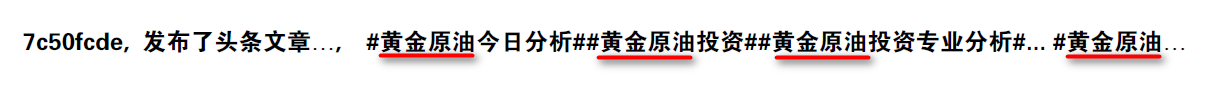
\includegraphics[width=\linewidth]{pic/prob3.png}
            \label{p3}
        \end{minipage}
    }

    \subfigure[标注问题]{
        \begin{minipage}[t]{\linewidth}
            \centering
            
\includegraphics[width=\linewidth]{pic/prob4.png}
            \label{p4}
        \end{minipage}
    }
    \vspace{-3mm}
    \caption{数据集部分问题图示{\label{H}}}
\end{figure}


\subsection{数据处理}
针对上述存在的问题,分别对应进行了如下处理:
\begin{enumerate}[label=(\roman*)]
    \item 用正则表达式进行模式匹配,删除脚本标记语言、特殊符号、重复符号等。
    \item 通过简单的文本相似性度量方法,剔除重复数据。对于标题和文本内容重叠的,舍弃标题不做处理。
    \item 找出标签所在上下文模式,剔除标签对文本带来的干扰。
    \item 对实验中观察到的有问题的数据,进行一部分重新标注。
\end{enumerate}
\par
在上述清洗数据的基础上,还会对文本进行多余空格的剔除。考虑到清洗过的数据以及一部分原始数据是没有标题的,对%
标题和文本内容进行合并处理。实验中因为用到了Bert模型,所以用额外的脚本将处理过的数据改写成相应的格式。

\section{算法与模型}
\subsection{Bert模型框架}
在参考文献\cite{devlin2018bert}\cite{2019albert}的基础上,我们选用Bert作为预训练模型。与之前的方法相比,该模型%
性能优越。报告\cite{devlin2018bert}中提出,Bert在机器阅读理解顶级水平测试SQuAD1.1中表现出惊人的成绩:全部两个衡量指标上全面超越人类,%
并且还在11种不同NLP测试中创出最佳成绩,包括将GLUE基准推至$80.4\%$(绝对改进7.6%),MultiNLI准确度达到$86.7\%$ (绝对改进率$5.6\%$)等。%
BERT模型是NLP领域发展的重大突破。\par

BERT全称Bidirectional Encoder Representations from Transformers。BERT的新语言表示模型,它代表Transformer的双向编码器表示。%
与最近的其他语言表示模型不同,BERT旨在通过联合调节所有层中的上下文来预先训练深度双向表示。因此,预训练的BERT表示可以通过一个额外的输出层进行微调,%
适用于广泛任务的最先进模型的构建,比如问答任务和语言推理,无需针对具体任务做大幅架构修改。图\ref{Comp_Bert} 展示了文献\cite{devlin2018bert}的结构。\par

\begin{figure}[!ht]
    \centering
    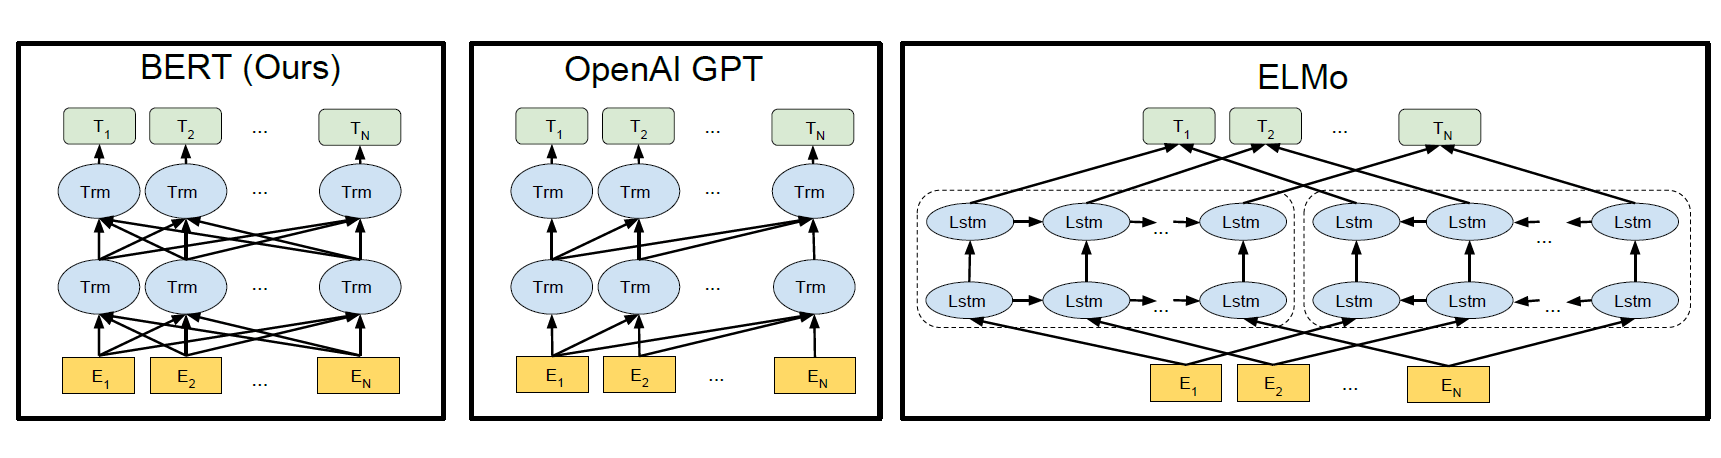
\includegraphics[width=\linewidth]{pic/Bert.png}
    \caption{Bert与其他模型的比较}
    \label{Comp_Bert}
\end{figure}

BERT的输入表示(input representation)能够在一个token序列中明确地表示单个文本句子或一对文本句子(例如, [Question, Answer])。对于给定token,A%
其输入表示通过对相应的token、segment和position embeddings进行求和来构造。图\ref{embedding}展示了这种输入表示。

\begin{figure}[!ht]
    \centering
    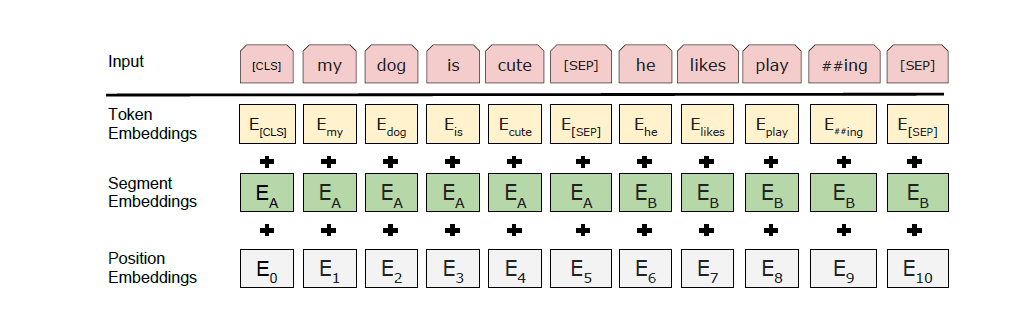
\includegraphics[width=\linewidth]{pic/embedding.png}
    \caption{Bert 输入表示}
    \label{embedding}
\end{figure}

\subsection{环境与配置}
互联网金融新实体发现是一个典型的NER问题。Google已经提供了关于中文语料的BERT预训练模型,所以我们选择了BERT模型来进行微调训练来实现我们的结果。 %
首先我们下载了BERT源码与关于中文的bert预训练模型(从BERT$-$Base Chinese下载模型 )。进行相关准备后,我们编写自定义的BERT\_NER.py文件,
参考bert源码中的run\_classifier.py。这一过程中,主要是定义DataProcessor和NerProcessor类,还有修改其他一些地方的引用关系,这是因为bert%
源码里面没有我们需要的专门的NER识别的操纵代码。编写时也参考了网上教程的改写方法。\par

在预训练的基础上,我们用处理后的数据集进行fine-tuning,训练100个epoch。代码已经上传到 \hyperref[code]{\texttt{\textcolor{blue}{Github}}} 存储库中,参数设置在json %
配置文件中,模型则上传到 \hyperref[code]{\texttt{\textcolor{blue}{OneDrive}}} 上。 

\section{结果分析}
\subsection{模型评估}
由于测试集没有标注数据,线上结果也未来得及及时更新,我们在报告中最终进行离线评估。具体的做法是将原训练数据分出一部分作为测试集并进行重新训练。按照官方给定的指标,分别计算准确率,召回率%
与相应的F Score。计算公式为
\begin{equation*}
    \begin{array}{l @{\; = \;} l}
        Precision & \displaystyle \frac{\sum_{i=1}^n TP_i}{\sum_{i=1}^nTP_i + \sum_{i=1}^nFP_{i}}, \\[20pt]
        Recall & \displaystyle \frac{\sum_{i=1}^n TP_i}{\sum_{i=1}^nTP_i + \sum_{i=1}^nFN_{i}}, \\[20pt]
        F \; Score & \displaystyle \frac{1}{1/Precision + 1/Recall}.
    \end{array}
\end{equation*}
其中,$n$为样本总数,$TP_i$是第ii条文本正确识别未知实体的数量,$FP_i$表示第i条文本中误识别为实体的数量,$FN_i$表示第i条文本中未识别出的未知实体数量。做评估时保留1k条数据,结果如表\ref{result} 所示。

\tabcolsep=20pt
\begin{table}[!ht]
    \centering
    \begin{tabular}{l l l l}
        \toprule
        Samples & Precision & Recall & F Score \\ \midrule
        1000    & 0.2634    & 0.2252    &  0.2409\\
        \bottomrule
    \end{tabular}
    \caption{评估结果}
    \label{result}
\end{table}

可以看到,最终的得分结果从指标上来说不尽人意。即便是得分比较高的队伍,线上得分也只在$0.3$至$0.4$之间。我们%
将一部分结果可视化,以作分析。结果如图\ref{results} 所示。\par
图\ref{r1} 展示了一个典型的相似实体误判的结果。“河南多家公司”与“河南高迈公司”比较相近,模型未能很好地作出区分。这导致了Precision指标的下降,%
而要用后处理来处理这样的结果,仍面临一定的困难。\par
图\ref{r2} 则是识别不精准的一个实例。与上一种情形相比,这种问题出现的频次相对少一些。在识别出的命名实体中,该例遗漏了“公司”两字,猜测可能是命名%
实体较长所致。这种情况下,在实际应用时不会带来很大影响,但Precision和Recall指标则会变成0。\par
图\ref{r3} 展示了误识别的一个例子。该例中的实体实际上是一个金融概念,但模型误识别为金融实体。这样的结果也很难作修正,因为在中文语境下,很多概念与实体是可以混淆的。\par%
图\ref{r4} 是典型的漏识别例子。注意到模型单独将标题断句为“文本”加以识别。这可能是漏识别的原因所在。
在模型预测阶段,除了上述的短句分句外,还有很大一部分只处理了文本的前128个字符。目前NLP的深度学习模型对长句的处理性能较差,所以对句长会有限制。由此带来的%
的漏判问题,我们还没有做很好的处理。

\vspace{-4mm}
\begin{figure}[!ht]
    \centering
    \subfigure[相似识别]{
        \begin{minipage}[t]{\linewidth}
            \centering
            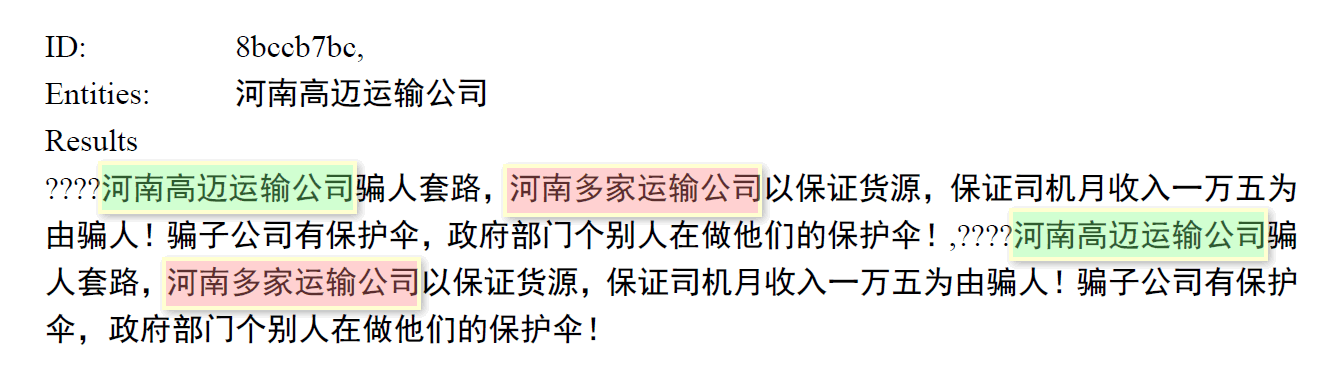
\includegraphics[width=\linewidth]{pic/result1.png}
            \label{r1}
        \end{minipage}
    }

    \subfigure[不精准识别]{
        \begin{minipage}[t]{\linewidth}
            \centering
            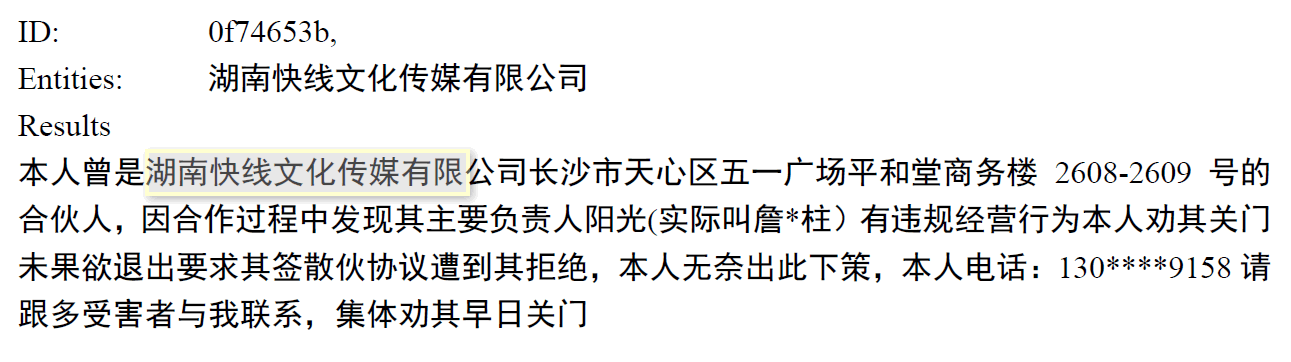
\includegraphics[width=\linewidth]{pic/result2.png}
            \label{r2}
        \end{minipage}
    }

    \subfigure[错识别]{
        \begin{minipage}[t]{\linewidth}
            \centering
            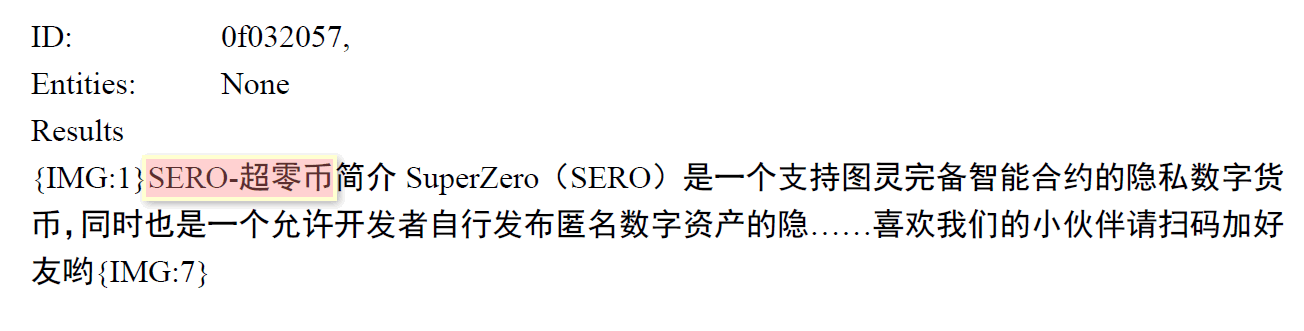
\includegraphics[width=\linewidth]{pic/result3.png}
            \label{r3}
        \end{minipage}
    }

    \subfigure[漏识别]{
        \begin{minipage}[t]{\linewidth}
            \centering
            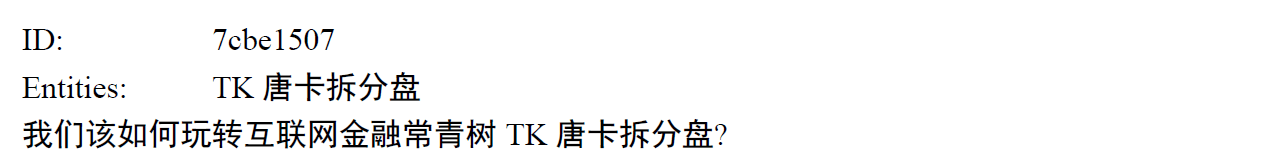
\includegraphics[width=\linewidth]{pic/result4.png}
            \label{r4}
        \end{minipage}
    }
    \vspace{-3mm}
    \caption{部分可视化结果问题图示{\label{H}}}
    \label{results}
\end{figure}

\subsection{模型展望}
文献\cite{2019albert}提出的Albert模型通过Embedding的处理和参数共享策略,降低了模型的规模,缩短了训练时间。如果改用Albert模型,有希望在同样的时间内进行更多的尝试,%
有潜力进一步提升性能。此外,由之前的结果分析,如果能通过一个混合模型对结果进行后处理,毫无疑问可以将指标提升很多。但是,这一模型本身也需要进行精心设计,目前没有找到%
比较有力的解决方案。在数据层面,可以通过进一步预处理,来解决Bert模型对长句的制约。

\bibliography{cite}
\bibliographystyle{ieeetr}

\section{附录}\label{code}
Our code is available \href{https://github.com/KAI-YUE/Financial-Entities-Recognition}{here}.\par
The model can be downloaded from \href{https://1drv.ms/u/s!AnzT-wEe9-ARgk4FviqmTab3qyCL?e=sSZOuU}{here}.\par
(Note: You may have to bypass GFW to get access to OneDrive.)

\tabcolsep=20pt
\begin{table}[!ht]
    \centering
    \begin{tabular}{ll}
        \toprule
        姓名  &  学号 \\    \midrule
        岳锴  &  PB16060757 \\
        廖云铭 & PB16060687 \\
        左琦  &  PB16061247 \\
        丁可  &  PB16061050 \\  \bottomrule
    \end{tabular}
    \caption{团队成员}
\end{table}

\end{document}